\documentclass[10pt]{article}

\usepackage[margin=0.65in]{geometry}
\usepackage{amsmath}
\usepackage{graphicx}
\usepackage{booktabs}
\usepackage{array}
\usepackage{hyperref}
\usepackage{microtype}

\title{\vspace{-1.4cm}Quick Report: Lean Floating-Point Stability Library and Benchmark}
\author{}
\date{May 8, 2026}

\begin{document}
\maketitle
\vspace{-1.2cm}

\section*{Purpose of the Library}

The project is a Lean 4 library for formally verified floating-point stability
analysis.  Conceptually, it is a formalization of Higham's book
\emph{Accuracy and Stability of Numerical Algorithms}: the goal is to turn
standard textbook stability results into reusable, machine-checked Lean
theorems.  It uses an abstract floating-point model rather than committing to a
particular IEEE standard: arithmetic operations are assumed to satisfy the usual
model
\[
  \mathrm{fl}(x \circ y) = (x \circ y)(1+\delta), \qquad |\delta| \leq u,
\]
where \(u\) is the unit roundoff.  This makes the library usable for any
floating-point system satisfying the model.

The library contains reusable definitions and theorems for error measures,
gamma bounds, summation, dot products, matrix-vector products, matrix
multiplication, triangular solves, LU analysis, QR/least-squares interfaces,
iterative refinement, perturbation theory, and related stability contracts.
Its intended use case is compositional stability analysis: instead of forcing a
human or AI agent to rederive all local floating-point error facts from first
principles, the agent can import the library, search its lookup documentation,
and assemble a machine-checked Lean proof of a target stability theorem.  This
is also relevant to autoformalization of numerical-analysis papers: if the
common floating-point machinery is already formalized, an AI agent can focus on
the paper-specific algorithmic argument rather than rebuilding the background
theory every time.

\section*{Benchmark Design}

The benchmark compares two settings on the same stability-analysis tasks.  In
the \emph{without-library} baseline, the agent receives only the minimal Lean
definitions needed for the theorem statement to parse.  In the
\emph{with-library} setting, the agent receives the full public library
snapshot, including documentation and examples.  In both settings, every
attempt runs in a fresh generated workspace with no memory from previous runs.
The theorem statement is the same, and the only accepted output is a Lean file
that builds and contains no \texttt{sorry}, \texttt{admit}, axioms, or
forbidden declarations.

Operationally, each task is a canonical Lean file containing the theorem to be
proved.  For every task, the harness creates two private directories under
\texttt{/tmp/lean-fp-benchmark-runs}: one for the without-library run and one
for the with-library run.  A dedicated workspace means that the solver sees
only that task package, its prompt, and the files intentionally exposed for the
condition.  It cannot reuse edits, memory files, or generated proofs from
previous tasks.  After the attempt, the temporary workspace is deleted and the
final Lean file, diff, logs, validation result, and metadata are copied back
into \texttt{benchmark/results}.

The with-library condition does not copy the whole project for every run.
Instead, the harness first builds a shared read-only public snapshot of the
library.  Each with-library task workspace is a small Lake package that depends
on this snapshot.  Thus the agent can inspect and import the public library,
but its edits are confined to the fresh task workspace.  The without-library
workspace resolves the same import names to small stub modules containing only
definitions, not the library's proved stability theorems.

The current experiment used ten externally motivated stability tasks.  Very
briefly, they cover LAPACK-style backward and forward error certificates,
residual stopping criteria, level-3 matrix multiplication, triangular residual
analysis, Oettli-Prager forward error, stationary iteration, least-squares via
QR, normal equations, and an Ogita-Rump-Oishi compensated summation
certificate.  These tasks are all stability-proof tasks: the goal is to prove
that a stated algorithm or certificate satisfies a numerical error bound.

\begin{table}[h]
\centering
\footnotesize
\begin{tabular}{p{0.12\linewidth}p{0.45\linewidth}p{0.32\linewidth}}
\toprule
Task & Stability example & Main source anchor \\
\midrule
E01 & LAPACK-style componentwise backward-error certificate from a computed residual. &
LAPACK Users' Guide, linear-equation error bounds; Oettli--Prager compatibility theorem. \\
E02 & Residual stopping criterion implying a relative forward-error target. &
Netlib Templates, stopping criteria for iterative methods. \\
E03 & LAPACK-style FERR forward-error bound using residual and inverse-magnitude data. &
LAPACK Users' Guide, linear-equation error bounds. \\
E04 & Normwise forward-error bound for computed matrix multiplication. &
LAPACK Users' Guide, fast Level 3 BLAS error bounds. \\
E05 & Residual bound for a computed triangular solve. &
LAPACK Users' Guide, fast Level 3 BLAS triangular-solve bound. \\
E06 & Oettli--Prager conversion from backward perturbations to forward error. &
Oettli--Prager 1964; LAPACK linear-equation error bounds. \\
E07 & Inexact stationary iteration residual recurrence and stopping analysis. &
Netlib Templates, stationary iterative methods and stopping criteria. \\
E08 & QR least-squares backward certificate converted to forward-error certificate. &
LAPACK least-squares error bounds; Bjorck least-squares survey. \\
E09 & Normal-equations perturbation certificate converted to forward-error bound. &
LAPACK least-squares error bounds. \\
E10 & SumK compensated-summation certificate proving an absolute error bound. &
Ogita--Rump--Oishi, \emph{Accurate Sum and Dot Product}. \\
\bottomrule
\end{tabular}
\caption{Benchmark examples.  Each task asks for a formal stability proof, not
just an algebraic simplification.}
\end{table}

The experiment reported here used:
\[
\text{model}=\texttt{gpt-5.5}, \qquad
\text{reasoning effort}=\texttt{xhigh},
\]
with persistent prompting and a 40 minute timeout per condition.  The prompt
explicitly told the agent not to stop after one failed proof route, and to keep
resolving Lean errors and remaining placeholders until \texttt{lake build
BenchmarkTask} succeeded or the external timeout stopped the attempt.
The command was \texttt{benchmark/scripts/run\_task\_once.sh <task>}, executed
with environment variables
\texttt{BENCHMARK\_CODEX\_MODEL=gpt-5.5},
\texttt{BENCHMARK\_CODEX\_REASONING\_EFFORT=xhigh},
\texttt{BENCHMARK\_SOLVER\_PROMPT\_VARIANT=persistent}, and
\texttt{BENCHMARK\_CODEX\_TIMEOUT\_SECONDS=2400}.  The run was executed
serially for E01--E10.  Inside each solver attempt, the agent was instructed
to edit only the proof body of \texttt{BenchmarkTask.lean} and repeatedly run
\texttt{lake build BenchmarkTask}.  The benchmark harness then performed an
independent validation build and rejected any remaining placeholder or
forbidden declaration.

The solver prompt was intentionally generic and did not reveal a task-specific
proof strategy.  Its essential instructions were: work only inside the current
workspace; replace the single \texttt{sorry} in \texttt{BenchmarkTask.lean};
do not change imports, definitions, namespaces, or the theorem statement; do
not add \texttt{axiom}, \texttt{opaque}, \texttt{unsafe}, \texttt{admit}, or
\texttt{sorry}; if \texttt{lake build BenchmarkTask} fails, read the Lean
errors and continue; only finish after a successful local build or after the
external timeout.  The with-library prompt allowed inspection of files already
present in the workspace, such as \texttt{public\_library}, \texttt{README.md},
\texttt{docs}, and \texttt{examples}; the without-library workspace simply did
not contain the full library snapshot.

\section*{Result}

All ten tasks passed in both conditions.  This is a strong result for the
library: access to the formalized stability library made the same proofs much
more scalable.  The with-library setting used about \(83.5\%\) less solver
time and produced proof bodies about \(81.3\%\) shorter on average.
Equivalently, the full library made the benchmark about \(6.1\times\) faster
in total solver time and about \(5.4\times\) smaller in final proof-body size.

\begin{table}[h]
\centering
\begin{tabular}{lrrr}
\toprule
Metric & Without library & With library & Reduction \\
\midrule
Total solver time & 155.84 min & 25.71 min & 83.5\% \\
Average solver time per task & 15.58 min & 2.57 min & 83.5\% \\
Average final proof body size & 254.4 lines & 47.5 lines & 81.3\% \\
\bottomrule
\end{tabular}
\caption{Aggregate results for the 40-minute persistent GPT-5.5 xhigh run.}
\end{table}

\begin{figure}[h]
\centering
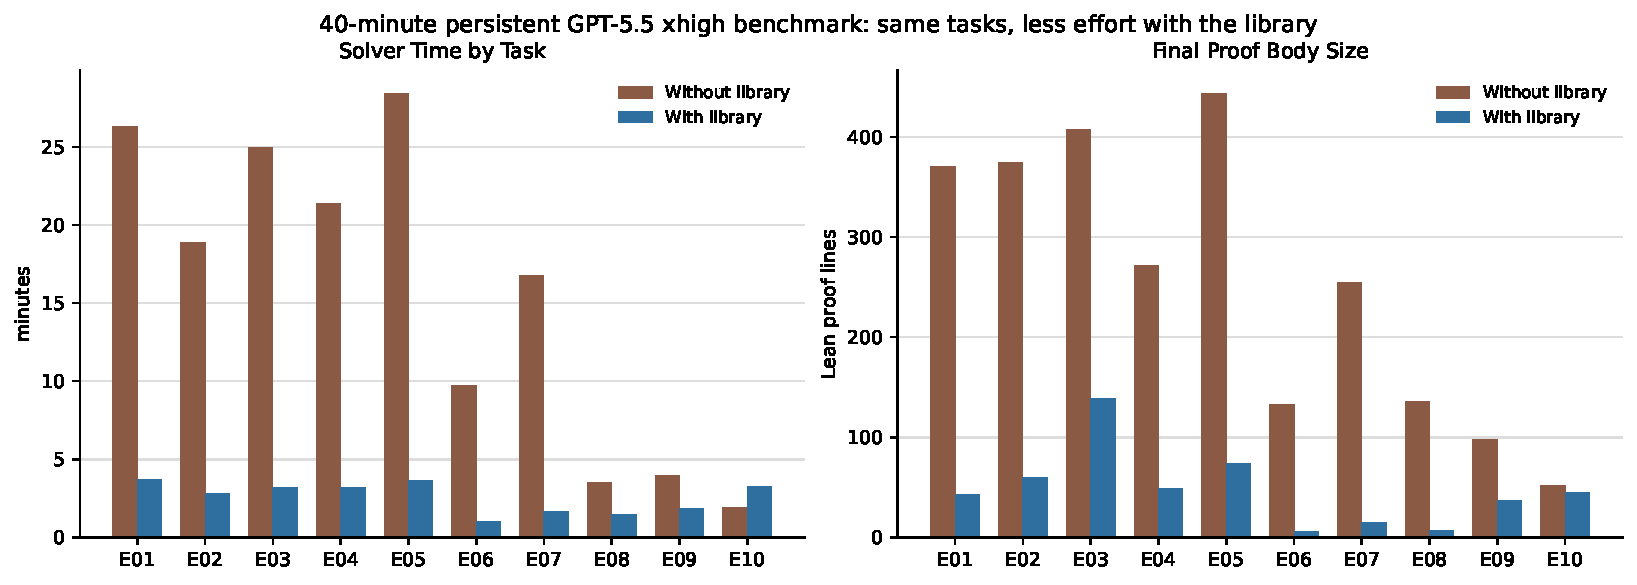
\includegraphics[width=\linewidth]{fig_discrepancy.pdf}
\caption{The library-assisted setting usually solved the same tasks much faster and with much
shorter proof bodies.}
\end{figure}

The only timing exception is E10, where the with-library run took slightly
longer.  This task is mostly a certificate-arithmetic inequality: the theorem
already exposes the key assumptions, so no major library theorem is needed.
The library-assisted agent spent extra time inspecting the larger library
surface, while still producing a slightly shorter proof.

\section*{Interpretation}

The main conclusion is that the library substantially improves automated
formal stability analysis.  Even when the agent is strong enough to eventually
solve all ten tasks without the library, it does so by spending much more time
and writing much longer local proofs.  With the library, the agent can reuse
formalized stability contracts and focus on composing them into the target
theorem.  This is the kind of improvement needed for scaling
autoformalization from isolated textbook examples toward scientific papers in
floating-point error analysis.

More and harder tasks should still be tested, especially tasks that require
deeper composition of stability results.  But the present result is already
positive: the Higham-style formal library gives a large practical reduction in
the effort required from the AI agent.

\section*{Source Anchors}

\footnotesize
The task statements were derived from external numerical-analysis or software
accuracy sources, then translated into Lean using the library's abstract
\texttt{FPModel} and \(\gamma\)-notation.  The main sources are:
LAPACK Users' Guide, ``Further Details: Error Bounds for Linear Equation
Solving'' (\url{https://www.netlib.org/lapack/lug/node81.html});
LAPACK Users' Guide, ``Error Bounds for Fast Level 3 BLAS''
(\url{https://www.netlib.org/lapack/lug/node108.html});
LAPACK Users' Guide, least-squares error bounds
(\url{https://www.netlib.org/lapack/lug/node82.html},
\url{https://www.netlib.org/lapack/lug/node83.html});
Netlib Templates, stationary methods and stopping criteria
(\url{https://www.netlib.org/templates/templates.html},
\url{https://netlib.org/linalg/old_html_templates/section2.8.2.html});
Oettli and Prager, ``Compatibility of Approximate Solution of Linear Equations
with Given Error Bounds for Coefficients and Right-Hand Sides'', \emph{Numerische
Mathematik} 6, 405--409, 1964 (\url{https://eudml.org/doc/131627});
Bjorck, ``The Calculation of Linear Least Squares Problems'', \emph{Acta
Numerica}, 2004
(\url{https://www.cambridge.org/core/journals/acta-numerica/article/calculation-of-linear-least-squares-problems/BA6F7F3457DA9172A313452C85E4702E});
and Ogita, Rump, and Oishi, ``Accurate Sum and Dot Product'', \emph{SIAM
Journal on Scientific Computing} 26(6), 1955--1988, 2005
(\url{https://ogilab.w.waseda.jp/ogita/math/doc/2005_OgRuOi.pdf}).

\end{document}
